\documentclass[a4paper,10pt,DIV10,openright,openbib]{scrreprt}
\usepackage[utf8]{inputenc}
\usepackage[T1]{fontenc}
\usepackage[english]{babel}
\usepackage[fixlanguage]{babelbib}
\selectbiblanguage{english}
\usepackage{float}
\usepackage{scrpage2}   %KOMA PG Settings
\usepackage{tocloft}    %ToC Control
\usepackage{graphicx}   %Better graphics
\usepackage{wrapfig}    %Better wrap text around figures
\usepackage[table,xcdraw]{xcolor}
\usepackage{array}      %Array Evironments (Matrices,etc)
\usepackage{tabularx}   %Better Tables
\usepackage{tikz}       %Tikz
\usepackage{pdfpages}   %Append PDF
\usepackage[english]{varioref}  %Intelligent page refs
\usepackage{makeidx}    %Index
\usepackage{listings}   %Better Listings
\usepackage{textcomp}   %Unicode Block
\usepackage{hyperref}   %Clickable links in .pdf
\usepackage{caption}    %Custom Caps in Floats
\usepackage{rotating}
\usepackage{mathtools}  %fancy arrows
\usepackage{amsmath}
\usepackage{amsfonts}
\usepackage{booktabs}
\usepackage{titling}
\setcounter{secnumdepth}{3}
\setcounter{tocdepth}{1}
\usepackage[stable]{footmisc}
\setlength{\textheight}{1.1\textheight} %BREAKS FOOTER?
% \usepackage{showframe} %DEBUG



% Bibliography no pagebreak:
\let\oldbibliography\bibliography% Store \bibliography in \oldbibliography
\renewcommand{\bibliography}[1]{{%
  \let\chapter\section% Copy \section over \chapter
  \oldbibliography{#1}}}% Old \bibliography


\RedeclareSectionCommand[
  beforeskip=-1.0\baselineskip,
  afterskip=-1\baselineskip]{subsection}
\RedeclareSectionCommand[
  beforeskip=-.75\baselineskip,
  afterskip=-1\baselineskip]{subsubsection}
\RedeclareSectionCommand[
  beforeskip=-2sp,
  afterskip=2\baselineskip]{chapter}
\makeindex
    \renewcommand{\abstractname}{System Background}
\usepackage{listings}
\usepackage{color}
 
\definecolor{codegreen}{rgb}{0,0.6,0}
\definecolor{codegray}{rgb}{0.5,0.5,0.5}
\definecolor{codepurple}{rgb}{0.58,0,0.82}
\definecolor{backcolour}{rgb}{0.95,0.95,0.92}
 
\lstdefinestyle{mystyle}{
    backgroundcolor=\color{backcolour},   
    commentstyle=\color{codegreen},
    keywordstyle=\color{magenta},
    numberstyle=\tiny\color{codegray},
    stringstyle=\color{codepurple},
    basicstyle=\footnotesize,
    breakatwhitespace=false,         
    breaklines=true,                 
    captionpos=b,                    
    keepspaces=true,                 
    numbers=left,                    
    numbersep=5pt,                  
    showspaces=false,                
    showstringspaces=false,
    showtabs=false,                  
    tabsize=2
}
 
\lstset{style=mystyle}

\begin{document}


%----------------------------
% Title
% ----------------------------
%titlepage
\thispagestyle{empty}
\begin{center}
\begin{minipage}{0.75\linewidth}
    \centering
%University logo
    
\includegraphics[width=120px,height=120px]{avatar-logo-blueonwhite.png} \\[0.3\baselineskip]
    \vspace{2cm}
%Thesis title
    {\uppercase{\Large System Design Project: \\ Project Plan\par}}
    \vspace{3cm}
%Author's name
    {\large Authors: \\
      Stefani Genkova   - \textit{s1437453} \\
      Tizzy MacGregor   - \textit{s1508959} \\
      Glen Merry        - \textit{s1531807} \\
      Alexander Pietz   - \textit{s1529373} \\
      Jasper Snel       - \textit{s1452790} \\
      Philip Van Biljon - \textit{s1545259} \\
      Boyan Yotov       - \textit{s1509922} \\
    \par} 
    \vspace{3cm}
%Degree
    {\Large DispensED - Group 17 \par}
    \vspace{3cm}
%Date
    {\small Last Update: \today}
\end{minipage}
\end{center}
\clearpage
%----------------------------
% /Title
%----------------------------
\newpage

\tableofcontents
% \listoffigures

\pagestyle{plain}
%\chapter{System Background}
%\section{System Description}

\section*{Purpose of this Document}
This document is prepared as part of the project for the System Design Project course
at the University of Edinburgh. The goal of the project is to build an assistive robot with 
appropriate software interface. Our project is to create a system that automates delivery 
of medicines to patients in care homes. This project plan will highlight the goals we
have set as a team, as well as how we will achieve them, and includes a breakdown
of our resources and an overview of our organisational structure.
\vspace{2cm}
{\let\clearpage\relax  \chapter{Introduction and Goals}}
% 3 marks ~1.5 pages
% The goal description should give an overview of the user problem and the robot
% task solution you propose. This could be in the form of a user story. If
% appropriate, include reference to existing systems that you are taking as
% inspiration, or published evidence for the user need that you plan to address.
% You should then breakdown the overall problem into the main technical
% subgoals, i.e., what you need to accomplish to get to the desired final
% result. For each subgoal you should provide an explicit milestone that states
% what you should have achieved, by what date, and what evidence you will
% present to show you have achieved it (e.g. a demonstration of the feature to
% your client).

There is a large shortage of nursing staff across the UK. The NHS reported in 2017
that nurses account for 38\% of overall vacancies in England \cite{NHS}.
The \textit{Care Home Use of Medication Study} has found that care home staff, specifically, spend about 40-50\% of their time with drug
related activities. The study also found that administration errors occur
8.4\% of the time \cite{CHUMS}, meaning that if a patient receives medication
three times a day, there is a 1 in 4 chance that an error will
occur\footnote{This can be viewed as Bernoulli experiment with 3 trials where the successive
  event is the correct administration of drugs. It follows that
  $\mathbb{P}(an\ error\ occurs) = 1 - \mathbb{P}(no\ error\ occurs) =
  \binom{3}{0}*0.916^3*0.084^0 \approx 0.23$}. \\
DispensED is aiming to develop a solution to the problems created by manual drug
administration by creating a robot to do the bulk of the work. Our product will
move around care homes to different residents' rooms. The residents can then
scan their identification and the appropriate drugs and vitamins will be
dispensed. The system will also have a wide range of administrative functions
available to staff, such as setting alerts on low stock levels or non-admittance of drugs.

\section{Technical Subgoals}
The system can roughly be divided into 4 parts, which will be desribed in this chapter, with different milestones set for each. The milestones are to be
presented at each demonstration, with the final demonstration being for the entire
system.

\subsection{Movement and Physical Frame}
The robot needs to be able to move around the facility in which it is deployed, using
motors mounted on a frame. The frame will also have to accommodate the other
physical parts of the system, and handle communication to the central system. 
The navigation will happen along predefined routes using marks on the floor. 
These marks are made using coloured tape.\\
%Additional care must be taken in regards to possible collisions as the robot
%will operate in a generally dynamic environment.
The different milestones for these can be set as follows:
\begin{enumerate}
  \item Initial control of simple frame with pre-programmed movement
  \item Full frame with pre-programmed movement
  \item Full frame with movement that is controlled by a remote computer
\end{enumerate}

\subsection{Dispensing of Medication}
The robot will support giving out medication that does not require a special environment
(for example requiring temperature control). It does this in two different ways:
\begin{itemize}
  \item \textbf{Pre Packed Sets of Medication} Most care homes get pharmaceutical drugs
pre-packed from the pharmacy, sorted by patient. In this case, the robot must
give out the container with the pre-packaged drugs to the correct patient. There
needs to be support for storing drugs for several different people who may not
collect their drugs in any predefined order.
  \item \textbf{Single Pills (Vitamins)} For pills that do not come pre-packed
(such as vitamins), a different kind of dispenser is needed. This dispenser must be able to hold a collection 
of a type of pill and give out single pills, one at a time.
\end{itemize}
Based on these two aspects, the following milestones can be set:
\begin{enumerate}
  \item Dispensing of individual (vitamin) pills
  \item Dispensing of pre-packaged pills for specific patients
  \item Recognising when the pills have been taken from the robot by the patient
    (dispensing tray empty)
\end{enumerate}

\subsection{Vision}
Several vision systems are needed in order for the robot to accomplish its objective:
\begin{itemize}
  \item \textbf{Orientation}
The robot must be able to recognise and process the markings on the floor that
are used for navigation. Additionally, the system must know the location of the rooms that
it is trying to service - separate floor markings or an alternative kind of
internal representation of the environment may be used for this.
  \item \textbf{Barcode Scanning}
Medication is dispensed to the patient after they have authorised themselves.
The main form of authorisation will be barcodes (these could be affixed to the
patients' wristbands). The system must be able to read these barcodes
\end{itemize}
This leads to the following milestones:
\begin{enumerate}
  \item Detecting target line and door markers
  \item Scanning barcodes and using them to report the ID of the patient
  \item Generating directions for actual movement: Using the lines to steer the
    robot along the lines.
\end{enumerate}

\subsection{Software Back- and Front-end}
To support the robot in getting the appropriate medication to patients, there will
be a back-end system in place, running on a central computer. This will hold a 
database of patients, medication, and what should be dispensed at which times. This, in
turn, will be accompanied by a user interface, which nursing staff can use to manage patients
and monitor what medication has been delivered. \\
This leads to the following milestones:
\begin{enumerate}
  \item A design plan of how the software will be structured. The current idea is to have a 
  modular design to maximise flexibility. This stage will also define the contents of 
  the different modules and how they will be approached.
  \item Implementation of database and software interface (API) to modify the database.
  \item Working user interface that inter-operates with the back-end
\end{enumerate}


%\subsection{Back-end}
%The back-end will offer a range of configuration as well as storing the patient
%database. Configured alerts will be sent out from the back-end, too.
%\subsubsection{Database} The Database will store patient information, including
%which room they reside in and their daily medication preferences. These
%preferences include:
%\begin{itemize}
%  \item Patient information
%  \item Type of medication needed (pre-packaged and/or loose?)
%  \item Deadline for drug admission (to send out alerts)
%\end{itemize}
%\subsubsection{User Interface} There will be a user interface to serve as the
%front-end to the aforementioned configuration.


{\let\clearpage\relax \chapter{Resource Allocation}}
% 3 marks for time planning ~1.5 pages
% 3 marks for identification of dependencies and risks ~1.5 pages
% The plan should explain how you will deploy your resources - 200 hours per
% group member over the semester - to achieve your goals. Note you should take
% into account time required by scheduled sessions (guest lectures, demo days,
% final presentations) and time used in planning and presenting (group meetings,
% report writing etc.), as well as time for building the system. You should also
% note the resources you have in terms of skills, equipment, etc. You must
% include a Gantt chart, which should clearly identify any dependencies between
% tasks. You may find it useful to make a revised version of your plan/gantt
% chart at key points in the project, in discussion with your client. The report
% should also contain an assessment of the risks that you anticipate for the
% project, and contingency planning that you have done to guard against them.

% Guest lectures: 8hrs 
% Demos and Pitches: 8hrs
% Planning and Presenting: 30hrs
% Development work: 150hrs
% Miscellaneous: 4hrs

\begin{wrapfigure}{r}{0.5\textwidth}
\centering
\begin{tabular}{@{}ll@{}}
\toprule
Team Member & Strengths                                                                                            \\ \midrule
Stefani     & \begin{tabular}[c]{@{}l@{}}Databases, Python,\\ Machine Learning\end{tabular}                               \\ \midrule[0.1pt]
Tizzy       & \begin{tabular}[c]{@{}l@{}}Object Oriented Programming,\\ Java, Database Management\end{tabular}                                                             \\ \midrule[0.1pt]
Glen        & \begin{tabular}[c]{@{}l@{}}Databases, Robot Construction,\\ Java, Python\end{tabular}                                                             \\ \midrule[0.1pt]
Alexander   & \begin{tabular}[c]{@{}l@{}}Project Management, LaTeX,\\ Python, Software Engineering\end{tabular}           \\ \midrule[0.1pt]
Jasper      & \begin{tabular}[c]{@{}l@{}}Vision, Program Design,\\ Object Oriented Programming\\Robotics Experience\end{tabular}                                                       \\ \midrule[0.1pt]
Philip      & \begin{tabular}[c]{@{}l@{}}Lego Mindstorm experience, Java,\\ Python, Language Processing \end{tabular}                                    \\ \midrule[0.1pt]
Boyan       & \begin{tabular}[c]{@{}l@{}}Electrical \& Mechanical Engineering,\\ Robot Construction, Physics\end{tabular} \\ \bottomrule
\end{tabular}
\caption{Team Strengths}
\label{skills}
\end{wrapfigure}

We first went and analysed particularly strong skills of our group members and how they might translate 
into out project. We have determined four core skills for each member (Table \ref{skills}). Next, we broke down
our project into smaller parts, each of which developed into a sub-team. We then assigned each team member 
to the sub-teams they were most interested in and where their strenghts would be most useful. For a full
list of the sub-teams, please refer to Table \ref{subt} in Section \ref{teamstr}.


\section{Time Planning}



The Gantt chart (Appendix 1) shows what should be done when, and who is responsible.
While we believe that Gantt charts are incredibly useful as tools to set goals and track
progress, we don't think this should dictate the entire project flow, especially considering
the highly flexible nature of the sub-teams. The focus will be on meeting the deadlines set
in the Gantt chart and analysing what resources should be dedicated to certain
tasks based on progress.\\
The deadlines for the milestones laid out previously are at the times of the client demonstrations (Milestone 1 = 
First client demonstration, ..). 
This means there will be plenty demonstrable material for every demonstration. Additionally,
after every demonstration, time has been scheduled to process any client feedback before the
next period of development starts.\\
We specifically left the period leading up to the final demonstration generic.
As this is a complex system with many parts, plenty of time is necessary to integrate them.
If there is time left over, then it will be used to expand functionality and polish up the final product.\\
\begin{figure}[h]
%   \centring
  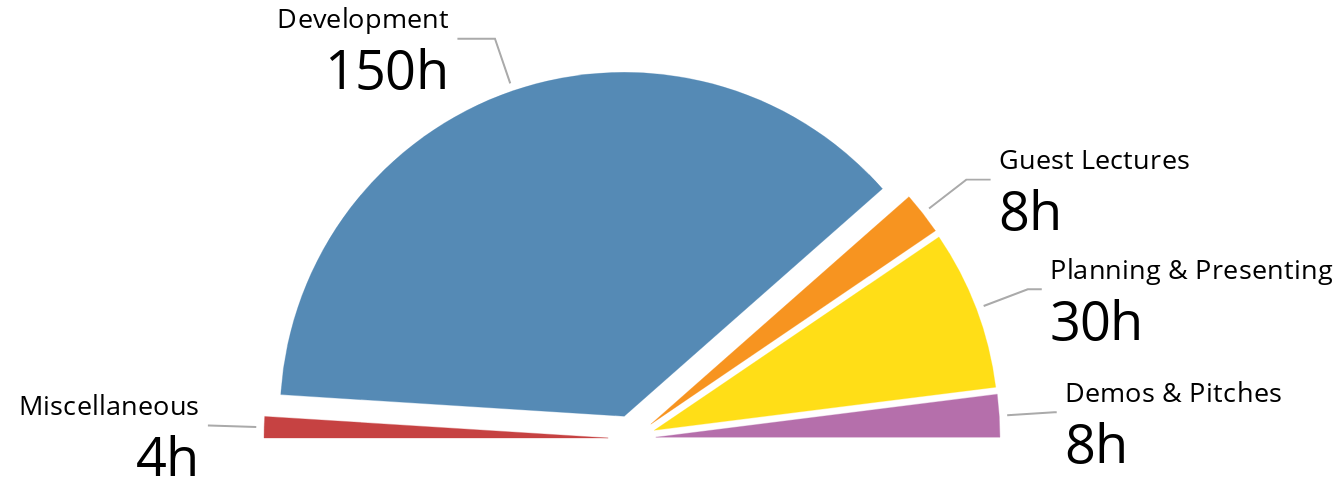
\includegraphics[width=\textwidth]{pie.png}
  \caption{Planned Individual Time Deployment}
  \label{piec}
\end{figure}
In terms of the total time to be spent on the project, the pie chart (Figure \ref{piec}) shows roughly how
much time per person is allocated to actual development of the system. This equates to around
14 hours per person per week. These can roughly be allocated to tasks. Every
team member
can then  compare their own contributions against those of others on the team, discussing any
problems in the regular meetings.

\section{Equipment and Physical Resources}
The robot will consist mainly of Lego while being controlled by the provided EV3 and Arduino kits. 
The only obvious thing that would have to be added to this is two cameras (for line detection and 
barcode scanning), and possibly 3D printed parts for medication dispensing. This should fit into 
the budget while leaving some room for additional parts where needed.
The software will run entirely on the provided DICE machine, meaning there is no need for additional
 resources.

\section{Risks and Contingency Planning}
The most apparent risk that would hinder project progress is absence of team members. 
As will be discussed in the next chapter, we split our team into multiple sub-teams. 
Every sub-team has multiple members and the project management ensures that no 
one team member has knowledge that no other 
team member possesses. This way, the impact of any one team member being ill or 
otherwise unable to work is minimised.\\
Other risks arise from needing to integrate 
the smaller parts of the system into one robot. We plan to use the time leading up to the final demonstration 
for this purpose, which should be adequate. It is still essential for the 
sub-teams to maintain regular communication with each other to make this process
as straightforward as possible. These and other identified risks have been
combined into the risk matrix \ref{risks} below.
\begin{table}[h]
  \centering 
\begin{tabular}{@{}llll@{}}
  \toprule
  Risk                                                                                                           & Likelyhood                   & Severity & Mitigation                                                                                                                                                                          \\ \midrule
  \begin{tabular}[c]{@{}l@{}}Team Members may be absent\\due to illness, etc\end{tabular}                       & \cellcolor{red!50} High     & \cellcolor{green!50} Low    & \begin{tabular}[c]{@{}l@{}}Division into sub-teams.\\ Multiple members in sub-teams create\\ redundancy. No one team member has \\ unique knowledge about the product.\end{tabular} \\ \midrule[0.1pt]
  \begin{tabular}[c]{@{}l@{}}Integration of sub-systems \\may be delayed if \\sub-systems are delayed\end{tabular} & \cellcolor{yellow!50} Medium & \cellcolor{red!50} High     & \begin{tabular}[c]{@{}l@{}}Regular communication between sub-\\teams ensures that they can maintain a\\ similar level of progress.\end{tabular}                                     \\ \midrule[0.1pt] 
\begin{tabular}[c]{@{}l@{}}Acquisition of critical items \\ may be delayed\end{tabular}                        & \cellcolor{green!50} Low     & \cellcolor{red!50} High     & \begin{tabular}[c]{@{}l@{}}Critical items must be ordered as soon\\ as possible.\end{tabular}                                                                                       \\ \midrule[0.1pt]
\begin{tabular}[c]{@{}l@{}}Support Staff may be unavailable\\ (Garry, Mentor, ..)\end{tabular}                 & \cellcolor{yellow!50} Medium & \cellcolor{yellow!50}Medium & \begin{tabular}[c]{@{}l@{}}Maintaining good progress towards our\\ milestones should minimise any \\last-minute support needs.\end{tabular}                                         \\ \midrule[0.1pt]
  Unrealistic Schedules                                                                                          & \cellcolor{yellow!50} Medium & \cellcolor{red!50}Low       & \begin{tabular}[c]{@{}l@{}}SCRUMBAN will enable us to re-plan\\ to meet deadlines accordingly\end{tabular}                                                                          \\ \midrule[0.1pt]
  Software compatibility issues                                                                                  & \cellcolor{green!50} Low     & \cellcolor{red!50}High      & \begin{tabular}[c]{@{}l@{}}Software is to be vigorously tested\\ on DICE \end{tabular}                                                                                               \\ \midrule[0.1pt]
User Interface unusable                                                                                        & \cellcolor{green!50} Low     & \cellcolor{green!50}Low     & Test UX with client prior to demo.                                                                                                           \\\bottomrule                                      
\end{tabular}
\caption{Identified Risks and their Mitigation}
\label{risks}
\end{table}

{\let\clearpage\relax \chapter{Organisational Structure}}\label{orgstr}
% 3 marks ~1.5 pages
% Finally, how you organise yourselves as a group and plan your work will be key
% to your success within the System Design project. You should detail the
% approach that you have taken to group organisation (e.g. specific roles of
% group members), meetings, communication, code-sharing, task allocation, and
% progress tracking.
\section{Team Structure}\label{teamstr}

\begin{table}[h]
\centering
\begin{tabular}{@{}llll@{}}
\toprule
Medication Dispensing & \begin{tabular}[c]{@{}l@{}}Software\\ Back \& Front End\end{tabular} &
\begin{tabular}[c]{@{}l@{}}Movement \\ (physical)\end{tabular} & Vision \\ \midrule
\textbf{Glen} & \textbf{Alex} & \textbf{Philip} & \textbf{Jasper} \\
Tizzy & Bobby & Jasper & Stefani \\
Philip & Glen & Bobby & \\
Stefani & Tizzy & Alex & \\ \bottomrule
\end{tabular}
\caption{Sub Teams - Key Contacts marked in \textbf{bold}.}
\label{subt}
\end{table}

The team structure loosely follows a Functional Matrix structure with Alexander
assigned as the key contact and team manager. As previously mentioned, we split our
team up into multiple sub-teams, (Table \ref{subt}) each working towards the sub-goals of their area. The
person marked in bold assigned as the ``owner'' of the groups work, meaning they are the first
point of contact.\\\\
The teams were created based on a combination of preference and competence, meaning each member will get to work on aspects they
find interesting and are most competent in. To ensure that the teams communicate effectively, each member is assigned to two
different teams, to create as much overlap between the teams as possible. This has the added benefit of ensuring that
each team has an understanding of the other parts of the system.\\
While the teams are inherently flexible, since members are on two teams simultaneously, there is also room for
movements between sub-teams. This could be due to unexpected workload, 
or if it turns out someone has valuable ideas for other aspects of the system. 
Any such shifts this would be discussed with the entire team.

\section{Meetings}
Every morning an informal stand-up is held so that everyone is able to be up to
date with the current state of the system. These catch-ups usually just include
any progress from the previous day as well as any potential new issues or roadblocks
that may have emerged.\\
The whole team meets with our mentor during a one hour fixed meeting slot on
Thursdays at noon - everyone is expected to attend these meetings. Quick
meetings will also happen directly after client demonstrations in order to
identify any issues that arose during the demo and plan to mitigate these in future.
Additional meetings follow a drop-in approach and are conducted as needed.
We will also meet after each demnstration to reflect on how it went and to plan
what needs to be improved before the next milestone.


\section{Communication and Tools}
The main vector of communication is the team Slack, while Notion is used as a platform for notes,
drafts and project management. Specific tasks are allocated via trello-like boards in
the To-Do section on Notion. We decided to use Notion instead of Trello as it
offers additional functionality. The way we manage both task allocation and
progress tracking follows SCRUMBAN management system, a mix between SCRUM
and KANBAN. This system picks out the most useful agile parts from KANBAN while
maintaining clearly defined roles. This will aid our team with more
steady progress whilst not locking ourselves into an engineering process that
requires planning very far ahead. \\
A private GitHub repository for code version control has been set
up for the project. We have used GitHub as it was the most accessible since
everyone already had an account.\\
\begin{table}[h]
\centering
\caption{Tool Overview}
\begin{tabular}{@{}lll@{}}
\toprule
Tool   & Purpose                                   & Link     \\ \midrule
Slack  & Main Communications HUB, Chat             & \url{https://sdpgroup17.slack.com/} \\
Notion & Meeting Notes, Project Management & \url{https://www.notion.so/dispensed/} \\
GitHub & Code Version Control                      & \url{https://github.com/xMythycle/DispensED/} \\ \bottomrule
\end{tabular}
\end{table}




%\bibliographystyle{alpha}
\bibliographystyle{alphadin}
\bibliography{Bibl}
%\begingroup
%\printindex 
%\endgroup

% Gantt Chart:
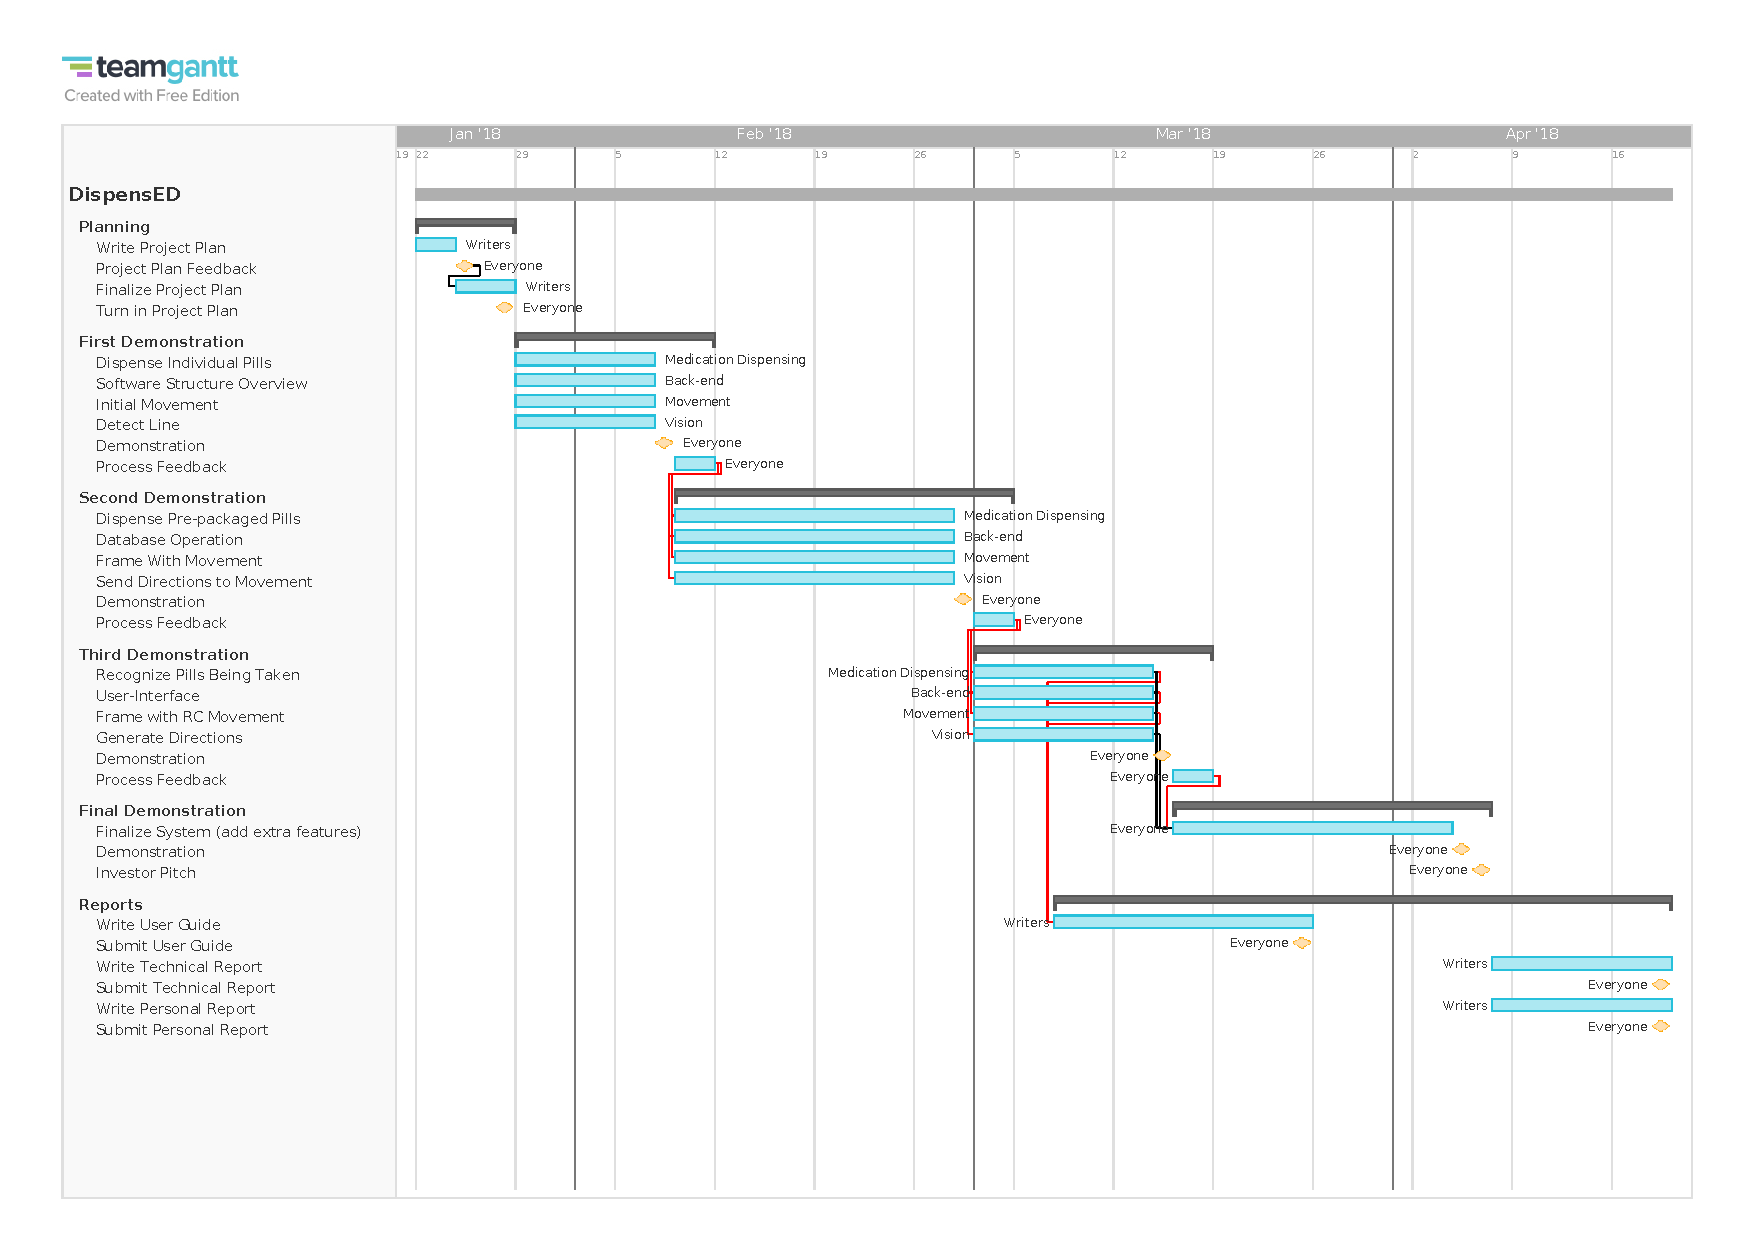
\includepdf[landscape=true]{gantt_chart}

\end{document}
